

\chapter{Návrh grafického uživatelského rozhraní}

    \begin{figure}[!h]
    \begin{center}
    \scalebox{0.5}{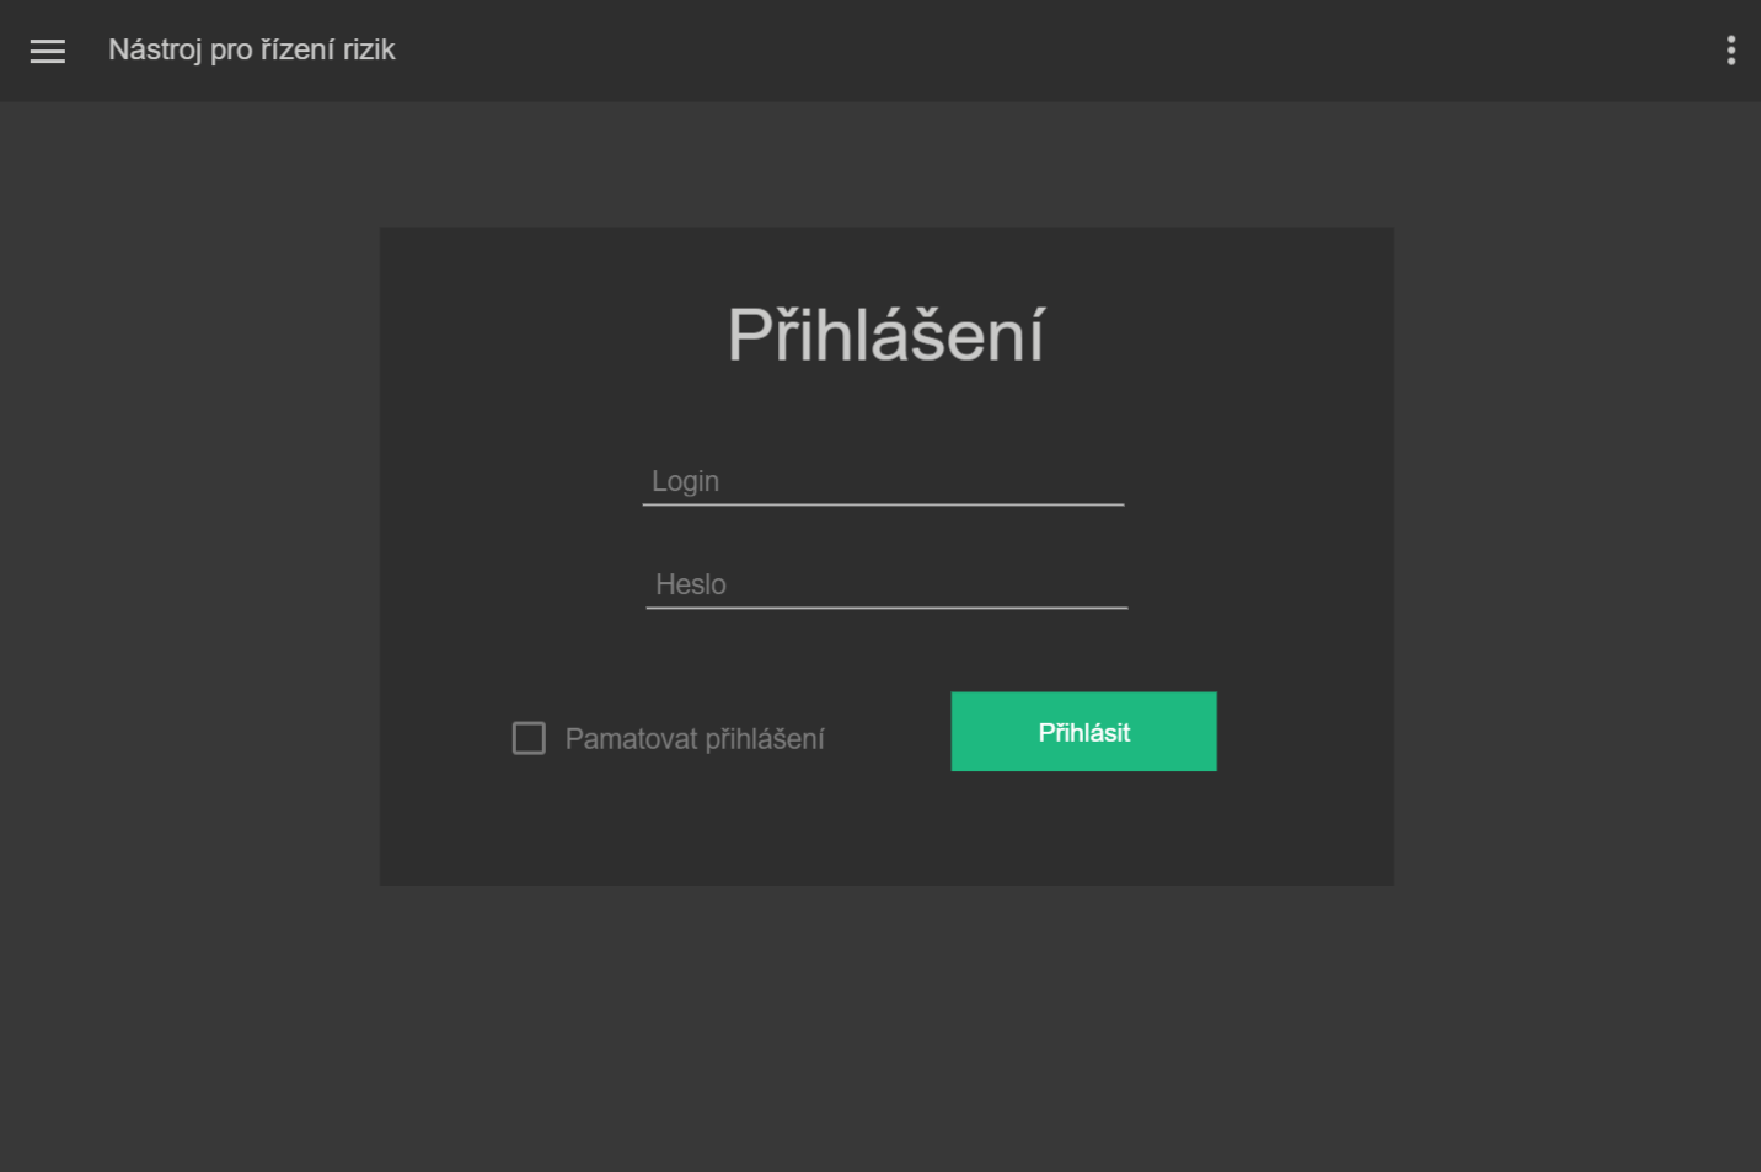
\includegraphics{obrazky-figures/Prihlaseni.pdf}}
    \caption{Návrh přihlašovácí stránky [zdroj vlastní]}
    \label{guiProjekt}
    \end{center}
    \end{figure}
    
    \begin{figure}[!h]
    \begin{center}
    \scalebox{0.5}{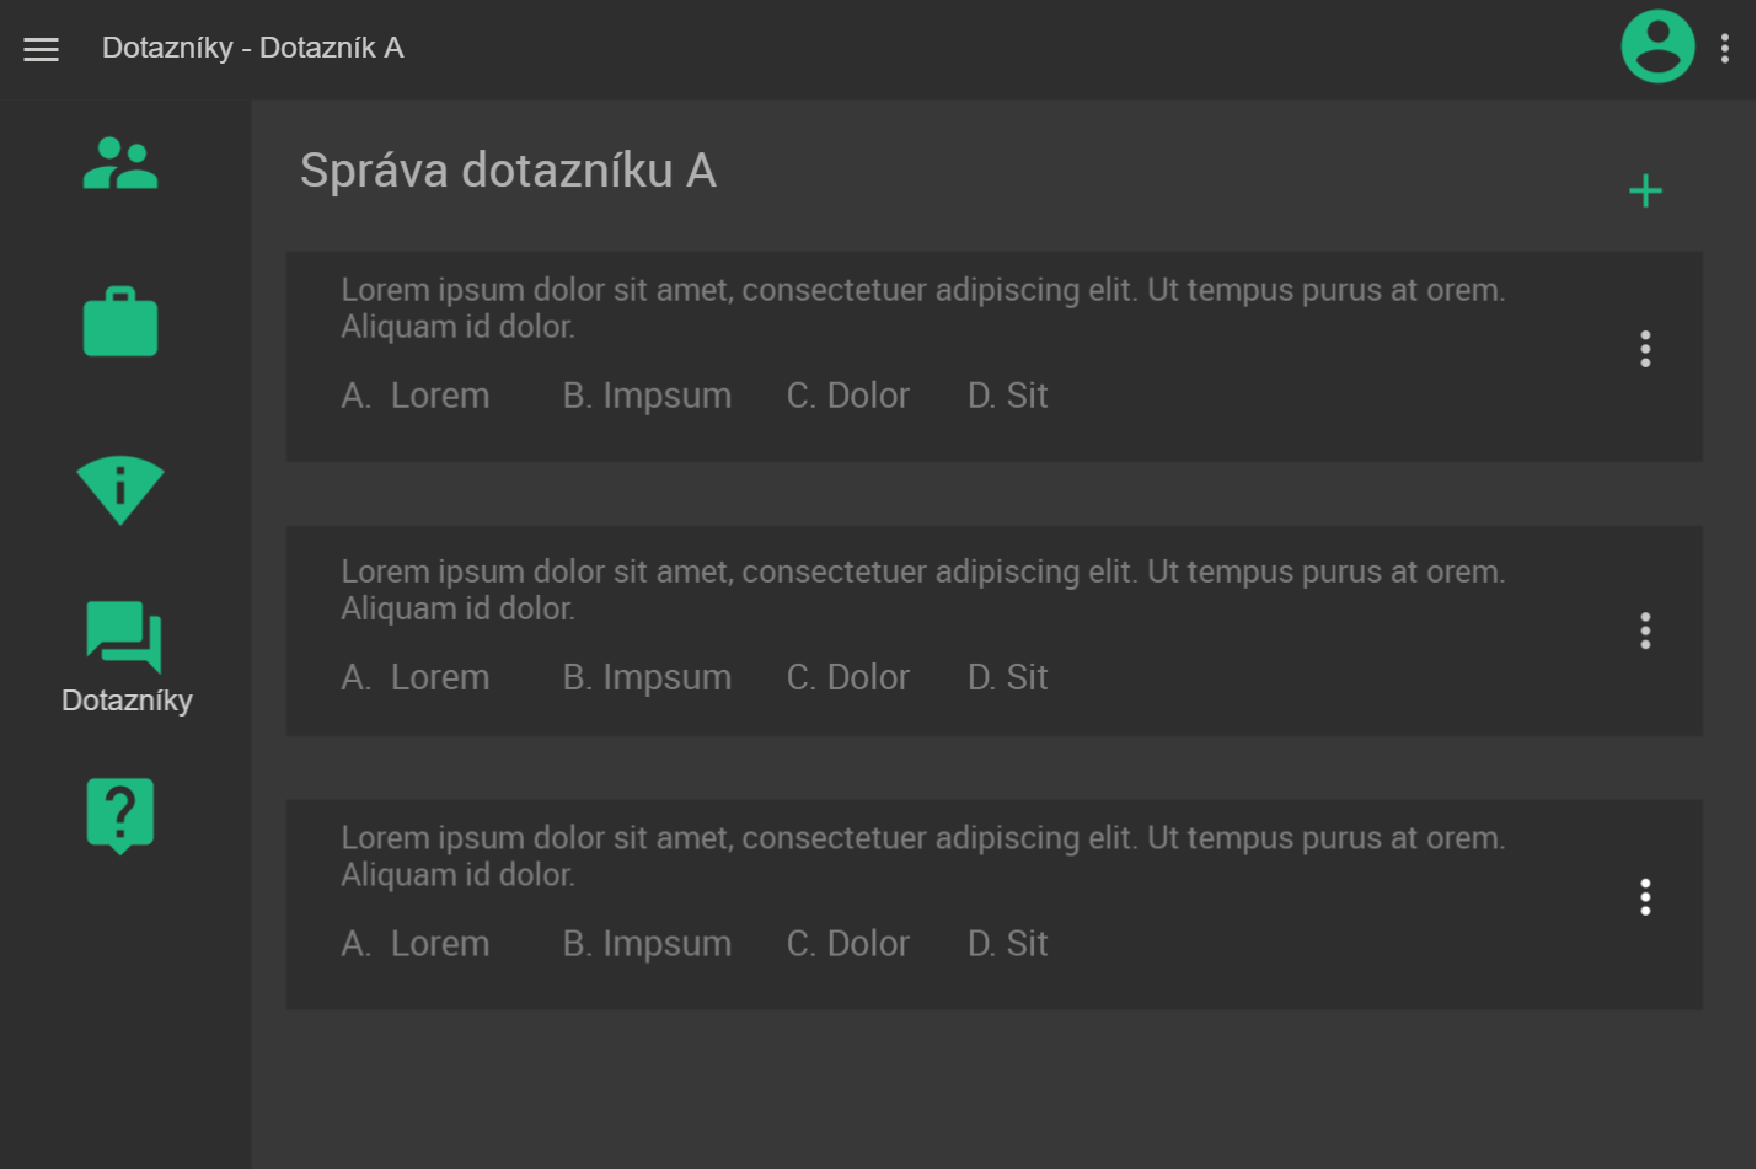
\includegraphics{obrazky-figures/SpravaDotaz.pdf}}
    \caption{Návrh stránky správy dotazníku [zdroj vlastní]}
    \label{guiProjekt}
    \end{center}
    \end{figure}

\chapter{API serveru}

Všechna URI mají předponu \texttt{api/nprr}.

\section{RoleController}
\begin{DESCRIPTION}
    \item \texttt{\textbf{POST /role}} Tvorba/editace role.
    \item \texttt{\textbf{GET /secRoles}} Získání všech bezpečnostních rolí.
    \item \texttt{\textbf{GET /secRole/{id}}} Získání bezpečnostní role dle jejího id.
    \item \texttt{\textbf{GET /roles}} Získání všech rolí.
    \item \texttt{\textbf{GET /role/{id}}} Získání role dle jejího id.
    \item \texttt{\textbf{DELETE /role/{id}}} Smazání role dle jejího id.
\end{DESCRIPTION}

\section{UzivatelController}
\begin{DESCRIPTION}
\item \texttt{\textbf{POST /user}} Tvorba/editace uživatele.
\item \texttt{\textbf{GET /users}} Získání všech uživatelů.
\item \texttt{\textbf{GET /info}} Získání informací o~aktuálně přihlašeném uživateli.
\item \texttt{\textbf{GET /users/count}} Počet záznamů v~tabulce s~uživateli.
\item \texttt{\textbf{GET /user/{id}}} Získání uživatele dle jeho id.
\item \texttt{\textbf{DELETE /user/{id}}} Smazání uživatele dle jeho id.
\end{DESCRIPTION}

\section{KategorieController}
\begin{DESCRIPTION}
\item \texttt{\textbf{POST /kategorie}} Tvorba/editace kategorie rizika.
\item \texttt{\textbf{GET /kategories}} Získání všech kategorií rizik.
\item \texttt{\textbf{GET /kategorie/{id}}} Získání kategorie rizika dle jejího id.
\item \texttt{\textbf{DELETE /kategorie/{id}}} Smazání kategorie rizika dle jejího id.
\end{DESCRIPTION}

\section{RegistrRizikController}
\begin{DESCRIPTION}
\item \texttt{\textbf{POST /risk}} Tvorba/editace rizika v~centrálním registru.
\item \texttt{\textbf{GET /risks}} Získání všech rizik z~centralního registru.
\item \texttt{\textbf{GET /risks/count}} Počet záznamů v~tabulce centralního registru rizik.
\item \texttt{\textbf{GET /risk/{id}}} Získání rizika dle jeho id.
\item \texttt{\textbf{DELETE /risk/{id}}} Smazání rizika dle jeho id.
\end{DESCRIPTION}

\section{OblastOtazkyController}
\begin{DESCRIPTION}
\item \texttt{\textbf{POST /questionArea}} Tvorba/editace oblasti otázky.
\item \texttt{\textbf{GET /questionAreas}} Získání všech oblastí.
\item \texttt{\textbf{GET /questionArea/{id}}} Získání oblasti otázky dle jejího id.
\item \texttt{\textbf{DELETE /questionArea/{id}}} Smazání oblasti otázky dle jejího id.
\end{DESCRIPTION}

\section{OdpovedController}
\begin{DESCRIPTION}
\item \texttt{\textbf{POST /answer}} Tvorba/editace oblasti otázky.
\item \texttt{\textbf{GET /answers}} Získání všech oblastí.
\item \texttt{\textbf{GET /answer/{id}}} Získání oblasti otázky dle jejího id.
\item \texttt{\textbf{DELETE /questionArea/{id}}} Smazání oblasti otázky dle jejího id.
\end{DESCRIPTION}

\section{OtazkaController}
\begin{DESCRIPTION}
\item \texttt{\textbf{POST /question}} Tvorba/editace otázky.
\item \texttt{\textbf{GET /questions}} Získání všech otázek.
\item \texttt{\textbf{GET /question/{id}}} Získání otázky dle jejího id.
\item \texttt{\textbf{DELETE /question/{id}}} Smazání otázky dle jejího id.
\end{DESCRIPTION}

\section{DotaznikController}
\begin{DESCRIPTION}
\item \texttt{\textbf{POST /survey}} Tvorba/editace dotazníku.
\item \texttt{\textbf{GET /surveys}} Získání všech dotazníků.
\item \texttt{\textbf{GET /surveys/cards}} Vrátí objekty karet dotazníků, které shnují jeho základní informace.
\item \texttt{\textbf{GET /survey/{id}}} Získání dotazníku dle jeho id.
\item \texttt{\textbf{DELETE /survey/{id}}} Smazání dotazníku dle jeho id.
\end{DESCRIPTION}

\section{ProjektController}
\begin{DESCRIPTION}
\item \texttt{\textbf{POST /project}} Tvorba/editace projektu - základní informace.
\item \texttt{\textbf{POST /project/survey}} Přiřazení dotazníku ke projektu.
\item \texttt{\textbf{POST /project/{idProj}/survey/{idSurv}/user/{idUser}}} Uložení do databáze informaci o~tom, jak uživatel odpověděl na daný dotazník na projektu.
\item \texttt{\textbf{POST /project/swot}} Tvorba/editace SWOT tabulky projektu.
\item \texttt{\textbf{POST /project/{id}/manager}} Přidání/změna manažera projektu.
\item \texttt{\textbf{POST /project/{id}/users}} Přidání/změna ostatních řešitelů projektu.
\item \texttt{\textbf{POST /project/{id}/risk}} Přiřazení rizika ke projektu.
\item \texttt{\textbf{GET /projects/active/user/{id}}} Získání modifikovaných objektů aktivních projektů, na kterých pracucje uživatel s~daným id. 
\item \texttt{\textbf{GET /projects/active/{isActive}/manager/{id}}} Získání modifikovaných objektů aktivních či neaktivních projektů, na kterých pracucje manažer s~daným id. 
\item \texttt{\textbf{GET /projects/active/{isActive}}} Získání modifikovaných objektů aktivních či neaktivních projektů.
\item \texttt{\textbf{GET /projects}} Získání všech projektů.
\item \texttt{\textbf{GET /projects/cards}} Získání objektů karet všech projektu, které shrnují jeho základní informace.
\item \texttt{\textbf{GET /projects/cards/user/{id}}} Získání objektů karet všech projektu, které shrnují jeho základní informace. Uživatel s~daným id je aktivním řešitelem nebo manažerem projektu.
\item \texttt{\textbf{GET /project/{id}}} Získání projektu s~daným id.
\item \texttt{\textbf{GET /project/{id}/users}} Získání všech aktivních i neaktivních řešitelů a manažerů projektu.
\item \texttt{\textbf{GET /project/{id}/survey}} Získání dat dotazníků, které se týkají projektu\,--\,jak uživatelé odpovídali na dotazník.
\item \texttt{\textbf{GET /project/{id}/risks}} Získání všech rizik přidělených projektu.
\item \texttt{\textbf{DELETE /project/{id}}} Smazání projektu dle jeho id.
\item \texttt{\textbf{DELETE /project/{id}/swot}} Smazání SWOT tabulky z~projektu dle jeho id.
\item \texttt{\textbf{DELETE /project/{id}/risk/{idRisk}}} Odebrání rizika z~projektu.
\item \texttt{\textbf{DELETE /project/{id}/survey}} Odebrání dotazníku z~projektu.
\end{DESCRIPTION}

\chapter{Použité knihovny při tvorbě klientské části}

Tento seznam, včetně verzí daných knihoven, lze najít v~souboru \texttt{package.json}.

\begin{DESCRIPTION}
\item \texttt{\textbf{date-fns a date-io/date-fns}} Date-fns zpřístupňuje metody pro manipulaci s~kalendářními daty. Date-io/date-fns pak tyto metody abstrahuje a díky tomu je můžou používat i jiné knihovny.
\item \texttt{\textbf{material-ui/core, material-ui/icons, material-ui/lab, material-ui/pickers}} \newline Jedná se o~různé části z~knihovny Material-UI. Core zpřístupňuje všechny komponenty, které tato knihovna obsahuje. Z~icons se pak přidávají Material Design ikony od společnosti Google. Lab obsahuje komponenty, které jsou ještě ve fázi testování a z~tohoto důvodu ještě nesou součásti balíčku core. Pickers se používají jako komponenty kalendáře a hodin.
\item \texttt{\textbf{nivo/bar, nivo/heatmap, nivo/pie }} Grafové komponenty z~knihovny Nivo. Nivo umožňuje stáhnout každý graf jako samostatnou knihovnu, aby výsledný balíček byl co nejmenší. Bar představuje sloupcový graf, pie je koláčovým grafem a modifikovaný heatmap se používá pro zobrazení matice pravděpodobnosti a dopadu. 
\item \texttt{\textbf{axios}} Knihovna, která hlavně umožňuje tvořit, posílat a přijímat HTTP požadavky.
\item \texttt{\textbf{formik}} Podpůrná knihovna pro jednodušší správu formulářů. Pro validaci používá knihovnu yup
\item \texttt{\textbf{yup}} Knihovna používá pro validaci dat v~nástroji. Lze použít pro validaci formulářů nebo i samostatných data.
\item \texttt{\textbf{material-table}} Tato knihovna tvoří komponenty tabulek, které jsou vytvořené ve stylu Material Desing. Vnitřně používá komponenty z~Material-UI
\item \texttt{\textbf{randomcolor}} Knihovna pro vygenerování náhodných barev. Používá se pro vybarveni grafů.
\item \texttt{\textbf{react a react-dom}} Jsou to balíčky z~knihovny React. Obsahují všechny potřebné komponenty pro vytvoření React aplikace. 
\item \texttt{\textbf{react-scripts}} Jde to balíček skriptů a konfiguračních souborů, které používá Create React App. Create React App se používá pro rychlé a automatické vytvoření výchozí React aplikace.
\item \texttt{\textbf{react-draggable}} Tvoří komponentu, díky které lze její potomky tzv. uchopit a přenášet. Používá se u~některých dialogů.
\item \texttt{\textbf{redux a react-redux}} Redux umožňuje vytvářet a spravovat globální stav aplikace a react-redux pak zpřístupňuje propojení mezi Reactem a Reduxem. 
\item \texttt{\textbf{redux-auth-wrapper}} Tato knihovna umožňuje definovat přístup k~jednotlivým částem aplikace podle role a oprávnění uživatele. Podobně pak omezuje přístup a viditelnost komponent. Není součástí systému Redux, ale využívá informace uložené v~globálním stavu. 
\item \texttt{\textbf{react-router-dom}} Propojuje DOM s~komponenty knihovny React Router. Díky tomuto lze v~aplikaci provádět směrování. 
\item \texttt{\textbf{react-promise-tracker}} Je to knihovna, která se používá pro sledovaní slibů (\textit{promise}) v~aplikaci. Díky tomuto je možné zobrazovat načítací obrázek v~době kdy se načítají data ze serveru.
\item \texttt{\textbf{react-swipeable-views}} Knihovna zpřístupňující komponentu pro plynulejší posouvání mezi stránkami na stejné úrovni. Je použita při odpovídání na dotazník projektu.
\end{DESCRIPTION}

\chapter{Testovací scénáře}